\qquad The TrackMe application has the following architecture. 
\begin{figure}[H]
	\begin{center}
		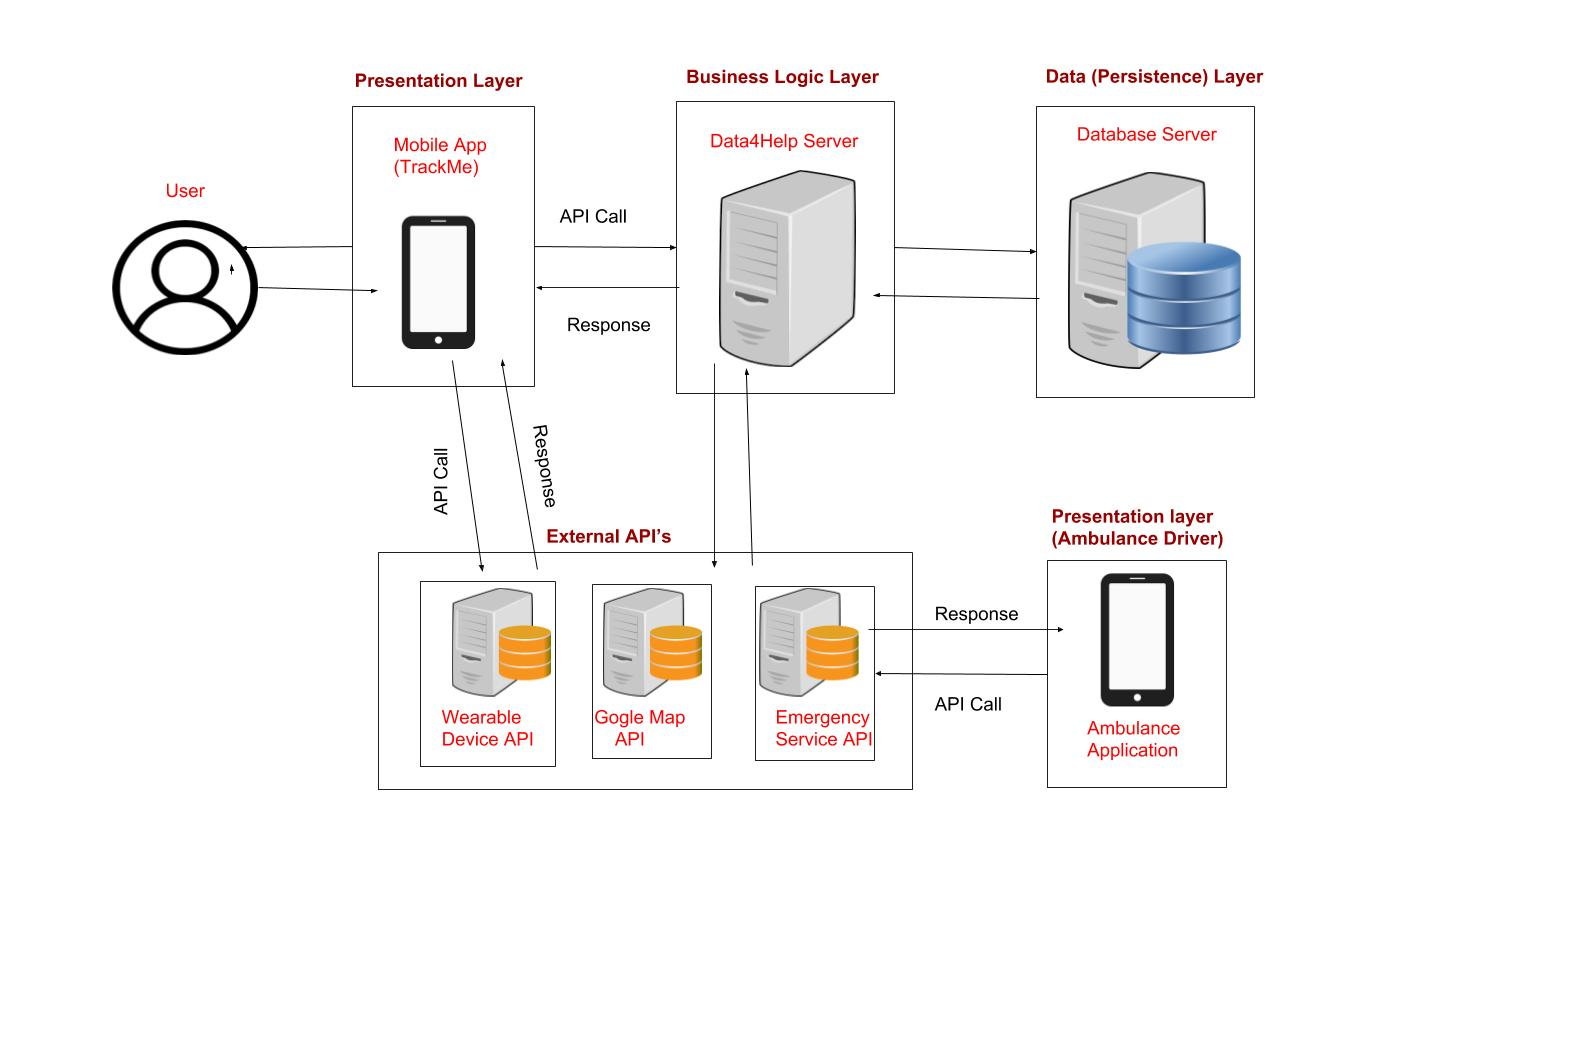
\includegraphics[width=\textwidth]{./DD_Diagrams/ArchitechuralView.jpg}
      	\caption{Architechtural overview of the system}
        \label{TrackMe_arc}
	\end{center}
\end{figure}
The architecture contains four layers, \textit{Presentation Layer}, \textit{Business Layer},\textit{ Data Layer} and \textit{External API's}. There are two presentation layer in the architecture as one is for the user and one explicit application for the ambulance driver so that they receive the individual's details within 5 seconds and can go to individual's location as soon as possible. All the layers are separately explained below:
\begin{itemize}
\item \textbf{Presentation Layer:} The presentation layer of the user provides a user interface to the third party and individual where they can perform operations. It also has a map which is used by users using the service of AutomatedSOS and Track4Run. The presentation layer takes the information from external API's by API call to display the information fetched from the external services in the user interface. It also has an API call from business logic layer to display the information from the database server of TrackMe which the user has given during registration.\newline
The presentation layer of the Ambulance Driver also uses external API's Google MAP API. It also uses the TrackMe server to receive Individual's location in the form of push notification.
\item\textbf{Business Logic Layer:} The business layer is the application server of the TrackMe application which manages the entire data flow from the application end to the data layer and vice versa. This layer focuses on the business front. and how it will be presented in front of the end users. This includes workflows, business components, and entities beneath the hood of two sub-layers named service and domain model layers.\newline
While the service layer focuses on defining a common set of application functions that will be available to users, the domain model layer represents expertise and knowledge linked to the specific problem domain. The entire plan is formulated in a way to explore and enhance the future of application. 
\item\textbf{Data (Persistence) Layer:} It contains all the data information which is required by the other layers of the system. It separates the getting and saving of the data from the business layer. The reason we do this is that the business logic (the part of the application that does the heavy lifting for your data manipulation) is not tied to a specific type of data source. The data layer will need to be written to be database specific.  This includes data access components, data helpers/utilities, and service agents.
\item \textbf{External API's:} This layer refers to all the external service used in the application. We use the API's of the external services in order to extract information from them and use it in the application. \textit{Wearable Device} is provided by the individual at the time of registering which they mention among all the list of compatible devices with the system. The API of the same wearable device is then used to extract the location and health information o the individual in order to provide them to the third party. The \textit{Google Map API} is used to display the map view in the application wherever it is required. The \textit{Emergency Service API} is used by the application to find the nearby hospitals and the ambulance they provide which can be used by the service of AutomatedSOS. 
\end{itemize}

 